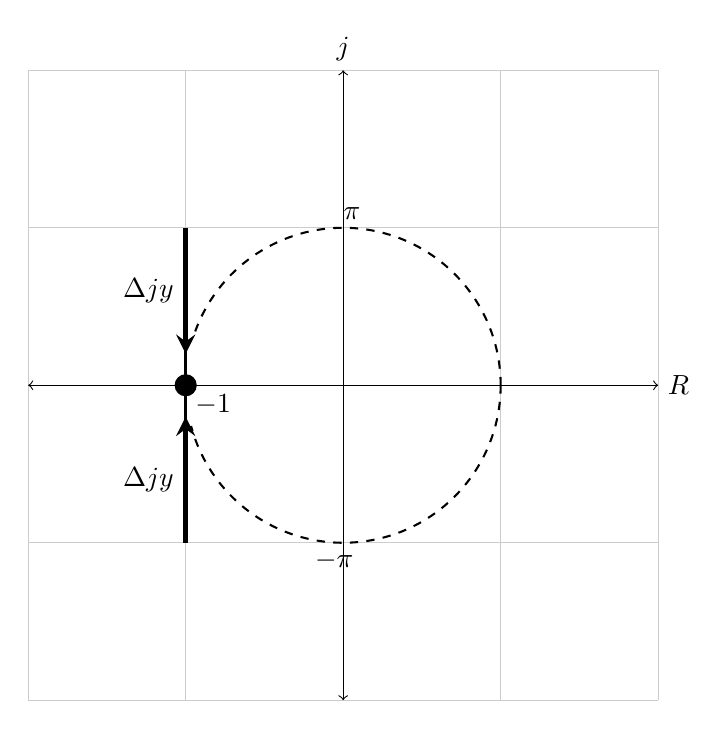
\begin{tikzpicture}[scale=2]
        \draw[thin,gray!40] (-2,-2) grid (2,2);
        \draw[<->] (-2,0)--(2,0) node[right] {$R$};
        \draw[<->] (0,-2)--(0,2) node[above]{$j$};
        \path[fill=black](-1,0) circle (2pt) node[anchor=north west]{$-1$};
        \draw[line width=0.75pt,black,dashed] (1,0) arc (0:160:1) node[midway, anchor=south east]{$\pi$};
        \draw[line width=0.75pt,black,dashed] (1,0) arc (0:-165:1) node[midway, anchor=north east]{$-\pi$};
        \draw[line width=2pt,-stealth](-1,1)--(-1,0.2) node[midway,left] {$\Delta jy$};
        \draw[line width=2pt,-stealth](-1,-1)--(-1,-0.2) node[midway,left] {$\Delta jy$};
        \draw[line width=1pt,-](-1,1)--(-1,-1);
\end{tikzpicture}
    \caption{Limite de la función $z^{1/2}$ en el punto $-1$}